\section{PERFORMANCE BENCHMARKS}

In this section we want to provide a number of performance benchmarks. The tests are running on an Intel i9-9980HK with a base clock of 2.4GHz and a burst clock of 5GHz. The CPU supports AVX, AVX2, and AVX-512.
The tests are running on a Dell Precision 7740 Workstation Laptop with 64GB RAM. As GPU we use an Nvidia RTX 3000 GPU. All benchmark tests were performed in Linux. For OpenCL on the GPU we use the Nvidia GPU drivers and as CPU runtime we compare the open-source POCL driver against the Intel CPU OpenCL runtime environment. All timing runs were repeated several times to make sure that the overhead from running the OpenCL and Numba JIT Compiler did not skew the results. Though hardly noticeable by users, for smaller experiments the JIT phase typically takes longer than the actual computation.

\subsection{Dense Operator assembly}

Let us start with benchmarking the dense operator assembly. We assemble the matrix $\dmat{A}$ defined by
$$
\dmat{A}_{ij} &= \int_{\Gamma}\psi_i(\bx)\int_{\Gamma}\frac{\phi_j(\by)}{4\pi |\bx -\by|}(\bx)\ds[\by]\ds[\bx]\\
$$
with $\Gamma$ being the unit sphere. For the basis functions $\phi_j$ and test functions $\psi_i$ we compare two cases, piecewise constant functions for both (P0 functions), or nodal, piecewise linear, and globally continuous functions for both (P1 functions). In the P0 case each triangle is associated with just one piecewise constant function. In the P1 case each triangle is associated with $3$ linear basis functions, one for each node of the triangle.

We first compare the OpenCL CPU performance for the Intel OpenCL runtime, and the POCL OpenCL runtime driver. We run the tests in single precision and double precision. The native vector width for both drivers in single precision is $8$, and and double precision $4$, which corresponds to AVX instructions. In Bempp-cl this means that we assemble in vectorized form one test triangle with $8$ trial triangles in single precision, and with $4$ trial triangles in double precision. Within the assembly almost all floating point instructions are manually vectorized to take advantage of this. We should hence see up a factor 2 speed-up between single and double precision assembly.



\begin{figure}
	\center
	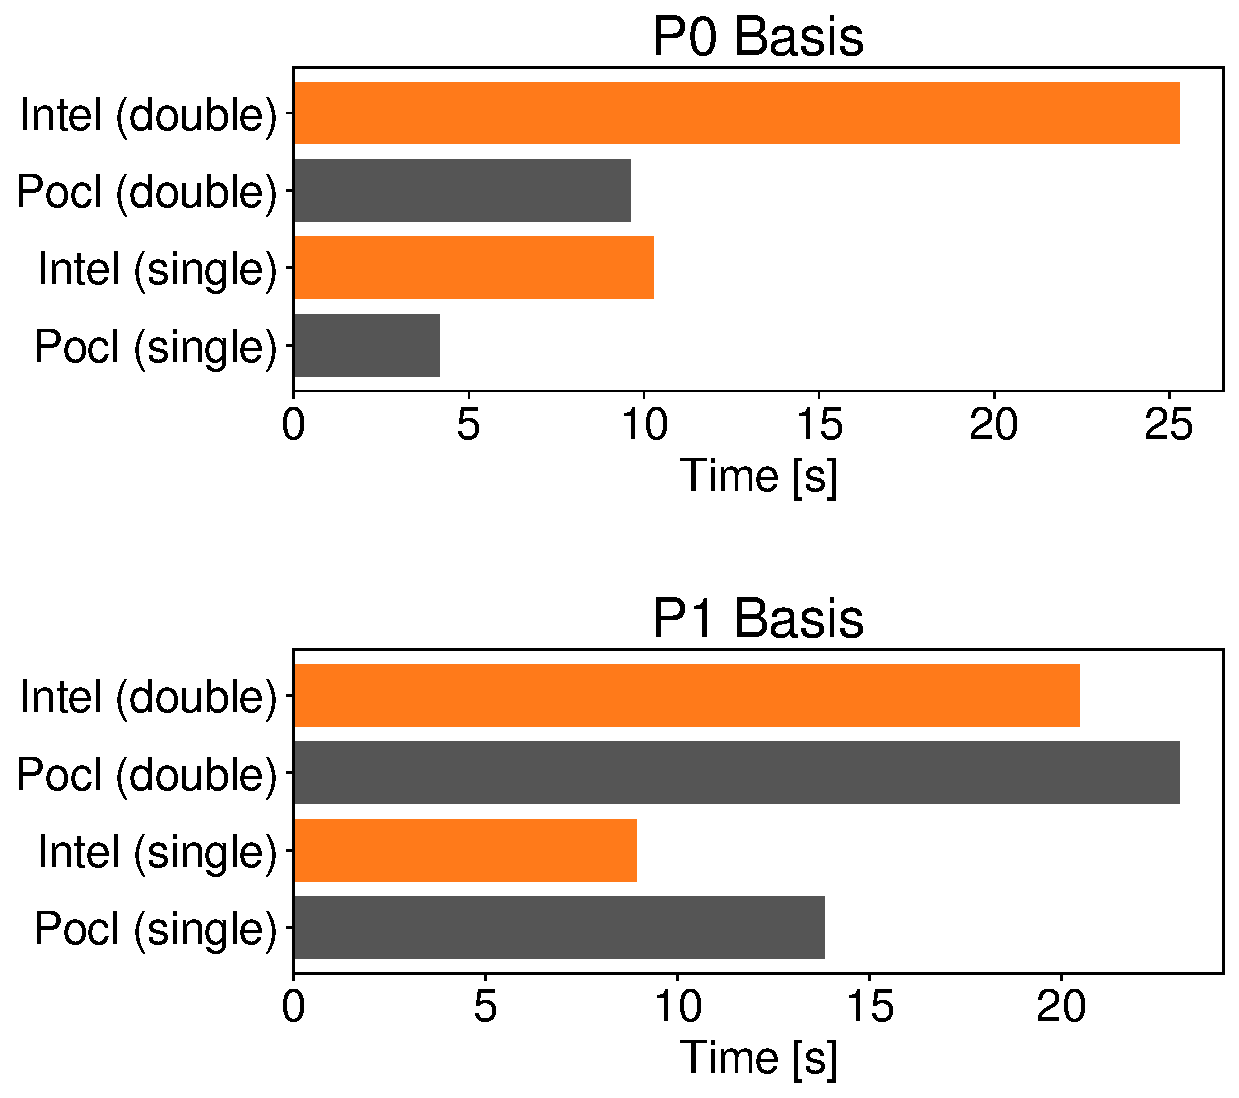
\includegraphics[width=6cm]{img/intel_pocl_laplace_comp.pdf}
	\caption{Comparison of the performance of POCL and the Intel OpenCL runtime for the assembly of the Laplace single-layer boundary operator on a grid with 32,768 elements.}
	\label{fig:intel_pocl_laplace_cmp}
\end{figure}

The results for a grid with 32,768 elements are shown in Figure \ref{fig:intel_pocl_laplace_cmp}. We see the expected speed-up between single precision and double precision evaluation. What is interesting to note is the difference between the Intel and the POCL runtime environment. For P0 basis functions the Pocl driver (black bar) significantly outperforms the Intel driver (blue bar) in both, single and double precision. For P1 basis functions the Intel driver gives better performance. The kernel source code is the same in both cases and manual vectorization of floating point operations is performed in the same way. However, in the P1 case significantly more data needs to be copied between a work-item and the global memory since the result of the interaction of a test triangle with a trial triangle is a local $3\times 3$ matrix containing all interactions between the three test basis functions on a triangle and the three trial basis functions. 

In Figure \ref{fig:pocl_single_layer} we compare specifically the performance of single precision and double precision evaluation for the POCL driver for various grid sizes in the case of a P0 basis. We can see that the speed-up for larger grid sizes is even slightly faster than just a factor two. The final data point in this graph corresponds to the grid size used for Figure \ref{fig:intel_pocl_laplace_cmp}.


\begin{figure}
	\center
	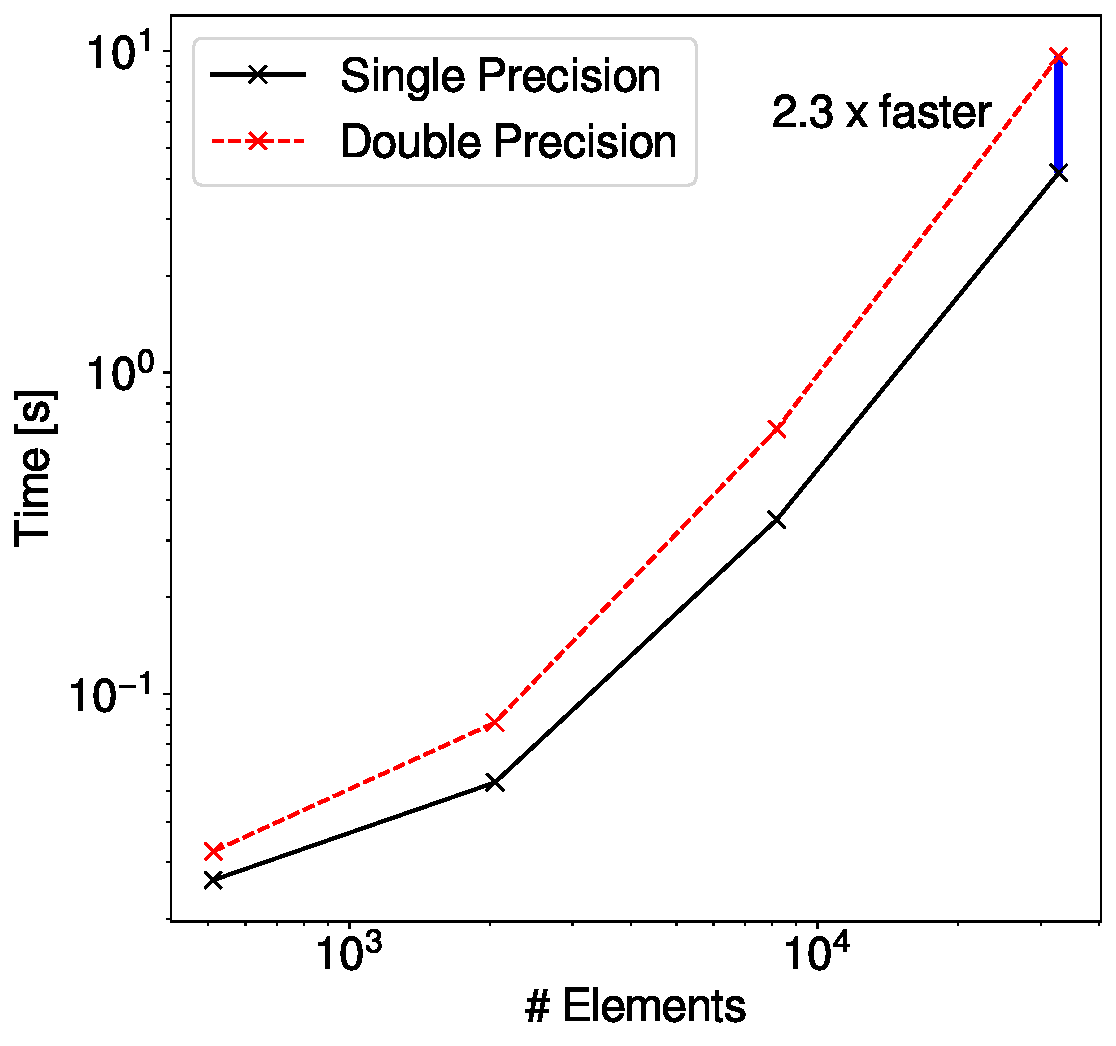
\includegraphics[width=7cm]{img/pocl_single_layer.pdf}
	\caption{Comparison of the single-precision and double-precision performance for various grid sizes using Pocl and P0 basis functions.}
	\label{fig:pocl_single_layer}
\end{figure}

In Bempp-cl we can easily switch between CPU Assembly, GPU Assembly and Numba Assembly. In Figure \ref{fig:cpu_gpu_numba_compare} we present a table for a grid size 2048 elements to compare these modes.
\begin{figure}
\begin{center}
\begin{tabular}{l|c|c}
	        &   single      &    double\\
	        \hline
	 POCL   &   0.05s       &    0.08s\\
	 Numba  &   0.25s       &    0.25s\\
	 GPU    &   0.11s       &    3s\\
\end{tabular}
\end{center}
\caption{Comparison of POCL, Numba and GPU Assembly for a grid with 2048 elements.}
\label{fig:cpu_gpu_numba_compare}
\end{figure}
The speed differences are striking. GPU assembly in single precision is a factor two slower than CPU assembly (and much slower in double precision due to Nvidia hardware restrictions for double precision). Numba is five times slower for single precision and still around three times slower for double precision than POCL. The GPU behaviour is due to the data transfer. We have done numerous experiments with GPU assembly of dense boundary integral operators. While the GPU kernels themselves are extremely fast, data transfer over the bus is destroying performance. But even for medium sized problems we have to transfer the data back to the main memory as GPU RAM is too limited to keep a number of dense matrices of dimension a few ten thousand on the device.

A different solution is to compute not the matrix but the matrix vector product $Ax$ on the device by recomputing all matrix elements in each-matvec on-the-fly but not storing them. We have done internal experiments with this and it gives significant speed-ups as compared to CPU evaluation as we now only need to transfer single vectors over the bus. But it is not competitive for larger problems compared to accelerated methods, such as Fast Multipole Methods due to the quadratic complexity of direct evaluation of the matvec as compared to linear complexity in the FMM. For smaller problem sizes it is still practically better to just assemble the whole matrix and store it, as then matvecs are much faster for an iterative solver. Hence, there is only limited practical relevance for such on-the-fly GPU evaluation of boundary integral operators. There is though very significant practical relevance of on-the-fly evaluation for the evaluation of domain potential operators for visualization and post-processing as we will see in the next section.

The Numba performance difference is interesting. The main issue, we think, is significantly less usage of AVX vectorized instructions. We have taken care to optimize the Green's function evaluation for vectorized evaluation. But the loops over integration points and other operations auto-vectorize very badly by just looping over all trial triangle for a single test triangle, as we currently do. We could tune our code for better auto-vectorization in Numba. However, this would be work with little benefit as we have highly optimized hand-tuned OpenCL kernels already. We therefore recommend Numba for operator assembly only as a fallback if no OpenCL runtime is available.

\subsection{Evaluating domain potentials for post-processing of electromagnetic problems}

Once an integral equation is solved one is usually interested in evaluating the solution not only at the boundary but also at points away from it. Hence, we want to evaluate
$$
f(\bx) = \int_{\Gamma}g(\bx), \by)\phi(\by) \ds[\by]
$$
for many points $\bx$ away from the boundary $\Gamma$. For example, if we want to visualize a solution the points $\bx$ would arise from some plotting grid. Typical of this operation that we usually only want to do it once or a few times at the end of a calculation. Discretising this operation into a dense matrix and then evaluating the dense matrix-vector product is not practical for larger sizes. For very large problems with hundreds of thousands of elements we use Fast Multipole or other accelerated approximate methods. However, for problem sizes of a few ten thousand elements up to around a hundred thousand elements (depending on the problem at hand), direct evaluation of this integral for every value $\bx$ is highly efficient. We won't go into the details of the corresponding OpenCL kernels here but want to show some results that demonstrate the performance of CPU vs GPU. While for the dense assembly of boundary integral operators the bus transfer of the dense matrix limited performance, here we only need to transfer to the device the vector of coefficients of the basis functions for $\phi$ and then back to the host the values at the points $x$.

For this section we used the evaluation of the electric potential operator, defined by
\begin{align*}
\mathcal{E\mathbf{p}}(\bx) &= ik\int_{\Gamma}\mathbf{p}(\by)g(\bx, \by) \ds[\by]\nonumber\\
&-\frac{1}{ik}\nabla_{\bx}\int_{\Gamma}\text{div}\,\mathbf{p}(\by)g(\bx, \by)\ds[\by]
\end{align*}
with $g(\bx, \by) = \frac{e^{ik|\bx - \by|}}{4\pi|\bx - \by}$ the Helmholtz Green's function, and
$k$ the wavenumber of the problem.
The function $\mathbf{p}(\by)\in\mathbb{R}^3$ is a vectorial function, leading to an overall vectorial solution at each point $\bx$. For details about the implementation of electromagnetic problems in Bempp see XXX. Here, we again use a grid with 32,768 elements and so-called (Rao, Wilton, and Glisson) edge based basis functions. We use 50,000 random evaluation points in the exterior of the unit sphere. We set $k=1.0$, though the value is not relevant for the performance.

In Figure \ref{fig:efield_domain_potential} we compare the performance of GPU evaluation with that of the POCL driver. In single-precision the GPU significantly outperforms the CPU, and even in double-precision the Quadro RTX is faster than the 8-core CPU, even though its hardware is not optimised for fast double-precision operations.

\begin{figure}
	\center
	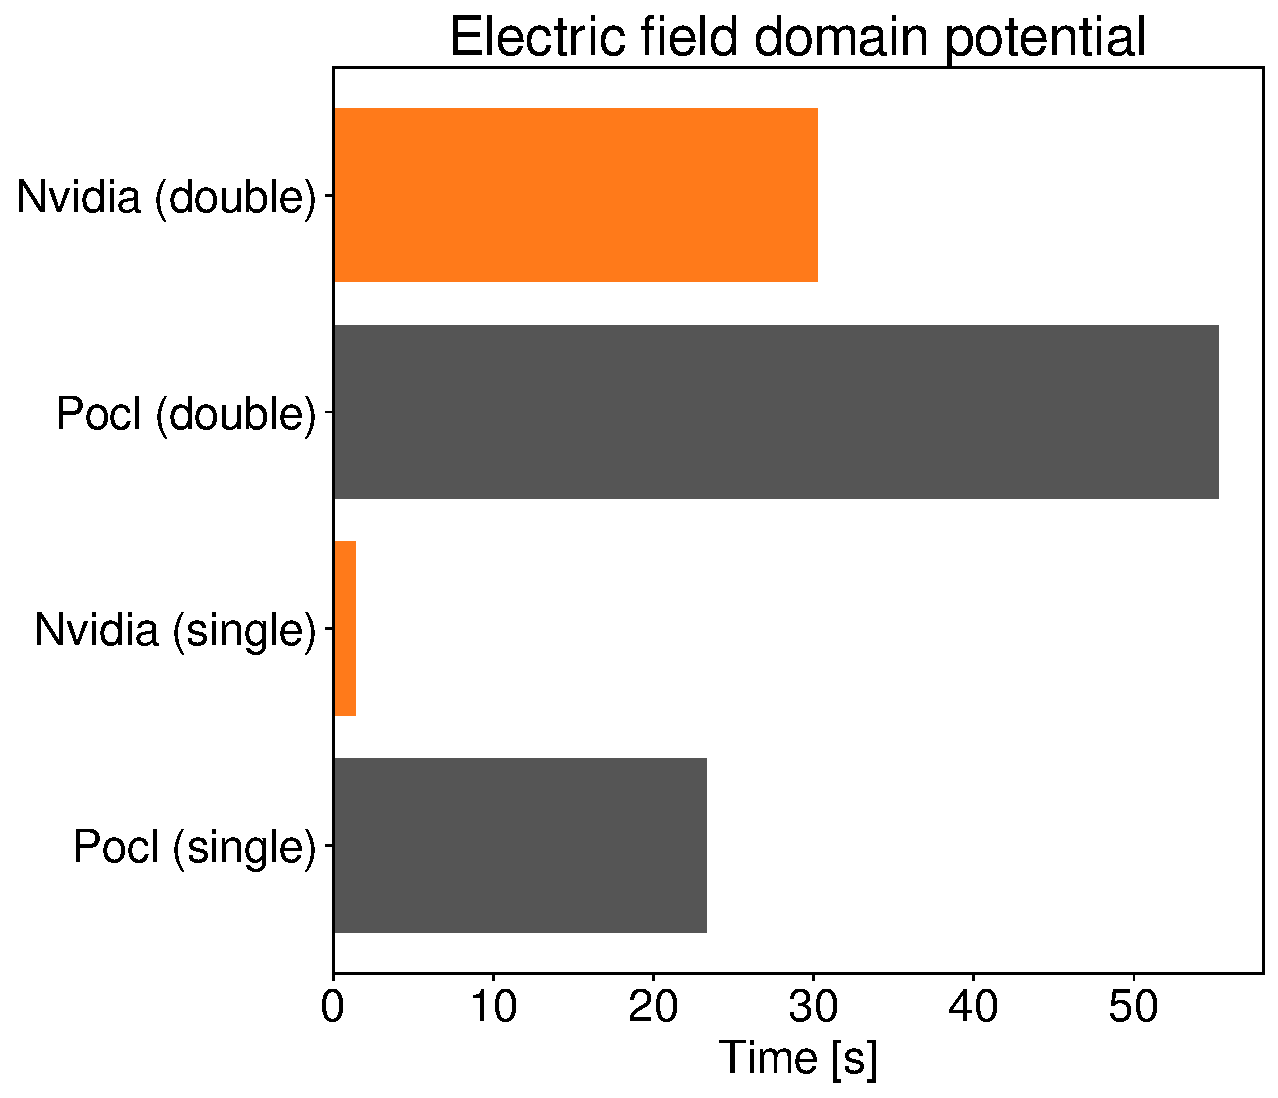
\includegraphics[width=7cm]{img/efield_domain_potential.pdf}
	\caption{Evaluation of an electric field potential operator on CPU via POCL vs GPU}
	\label{fig:efield_domain_potential}
\end{figure}

\section{SUMMARY}

With Bempp-cl we have created a Python platform that achieves high-performance through use of modern JIT technologies. Bempp-cl mixes Numba evaluation for less compute intensive linear complexity loops and sparse matrix generation with highly optimized OpenCL kernels for computationally sensitive dense matrix assembly routines. Basing development on Python instead of classical C/C++ makes it very easy to adapt the library and integrate into other applications with Python interfaces. An example is the recent work of integrating Bempp-cl and the Exafmm library for electrostatic virus-scale simulations [XXX]. Strict separation of the computational backend from the interface layer in the library also makes it easy to integrate further backends. We currently support Numba and OpenCL as compute backends. Other technologies could be added easily. OpenCL itself has proved a valuable choice for the purpose of this library. We have all kernels available in CPU and GPU optimized versions and the user can easily move between CPU and GPU based compute devices by a simple parameter change, allowing us to support a wide range of hardware. Here, we have demonstrated Nvidia benchmarks. But it would have made no difference to use AMD or Intel GPUs.

A disadvantage of our approach is that using OpenCL kernels is mixed-language development due to the OpenCL kernels written in C99. Using Numba throughout would be a much more native Python experience. However, while Numba is constantly improving, achieving optimal performance for complex operations is difficult. OpenCL shines here. It makes explicit SIMD operations very easy through dedicated constructs. Moreoever, OpenCL kernels are completely stack based functions, allowing much better optimisations while Numba needs to create every object dynamically, even very small arrays for objects such as coordinate vectors.

Also, one has to consider for this approach the type of operations that are required to be accelerated. For the dense assembly of integral operators we have very simple data structures that can easily be passed to compute kernels. More complex data structures with larger mixture of data movement operations and computations (e.g. tree-based algorithms), are much harder to accelerate since the Python layer imposes limits here on the performance.

Overall, with the model of mixed Python/OpenCL/Numba development we have created a flexible and easy to extend platform for integral equation computations and it was an effort that has payed back in terms of simple development without sacrificing performance. Strict separation of compute backends and higher level routines makes it easy for us to integrate other accelerator techniques in the future with little code changes, and to react to new trends in heterogeneous computing.

The current focus of further developments is on MPI implementations for cluster computing via \verb@mpi4py@. We have also made big steps forward for large problems by creating a black-box FMM interface that is currently implemented for Exafmm, which has allowed us to solve problems with 10 million elements on a single workstation. This shows that Python focused development (with some native routines in lower-level languages) is a scalable model and we are aiming to exploit this scalable further as we move from single workstation computations to large cluster problems.